\documentclass{rjparticle}
\usepackage{graphicx}
\usepackage{lipsum}

\title{Extensive Study of the Wobbling Properties in $^{163}$Lu Based on the Parity Concept} 

\author[1,2,$a$]{Robert Poenaru}

\author[1,3,$b$]{Apolodor Aristotel Raduta}

\affil[1]{``Horia Hulubei'' National R\&D Institute for Physics and Nuclear Engineering,\\
Reactorului 30, RO-077125, P.O.B. MG-6, M\u{a}gurele-Bucharest, Romania
\email[a]{robert.poenaru@drd.unibuc.ro} (corresponding author)}
\affil[1]{``Horia Hulubei'' National R\&D Institute for Physics and Nuclear Engineering,\\
Reactorului 30, RO-077125, P.O.B. MG-6, M\u{a}gurele-Bucharest, Romania}
\affil[2]{Doctoral School of Physics, University of Bucharest, Romania}
\affil[3]{Academy of Romanian Scientists, Bucharest, Romania\\
\email[b]{raduta@nipne.ro}}


\keywords{Wobbling Motion, Nuclear Structure, Parity Symmetry}

\bibliographystyle{plain}

\begin{document}

\maketitle

\begin{abstract}
A new interpretation on the wobbling structure in $^{163}$Lu is developed, based on the concept of parity symmetry. It is known that four wobbling bands are experimentally observed in this isotope, where three of them are considered as wobbling phonon excitations (namely $TSD_2$, $TSD_3$, and $TSD_4$) and the yrast band for the ground state (that is TSD1). In the present work, the trial function that is used for obtaining the wobbling spectrum is analyzed in terms of its behavior under the rotation operation. Indeed, due to a specific symmetry to rotations with $\pi$ around the 2-axis of the triaxial system, the parity becomes a good quantum number. As such, the trial function admits solutions with negative parity, which belong to the rotational states in $TSD_4$. A unified description of all the triaxial super-deformed bands in $^{163}$Lu is achieved with the new formalism.
\end{abstract}

\section{Introduction}
Wobbling motion in nuclei was extensively studied in the recent years, and the scientific community finally shed some light on this elusive phenomenon. This kind of collective motion was firstly predicted by Bohr and Mottelson, more than 50 years ago \cite{bohr1998nuclear}.

\section{Theoretical Background}

In a previous work, a complete description of the triaxial characteristics of the Lu isotopes was given, where results for the wobbling energies and transition probabilities were presented \cite{raduta2018wobbling}.

In this paper, the wobbling spectrum is represented. See Figure \ref{tsd_spectrum} for more details.

\begin{figure}[ht]
    \centering
    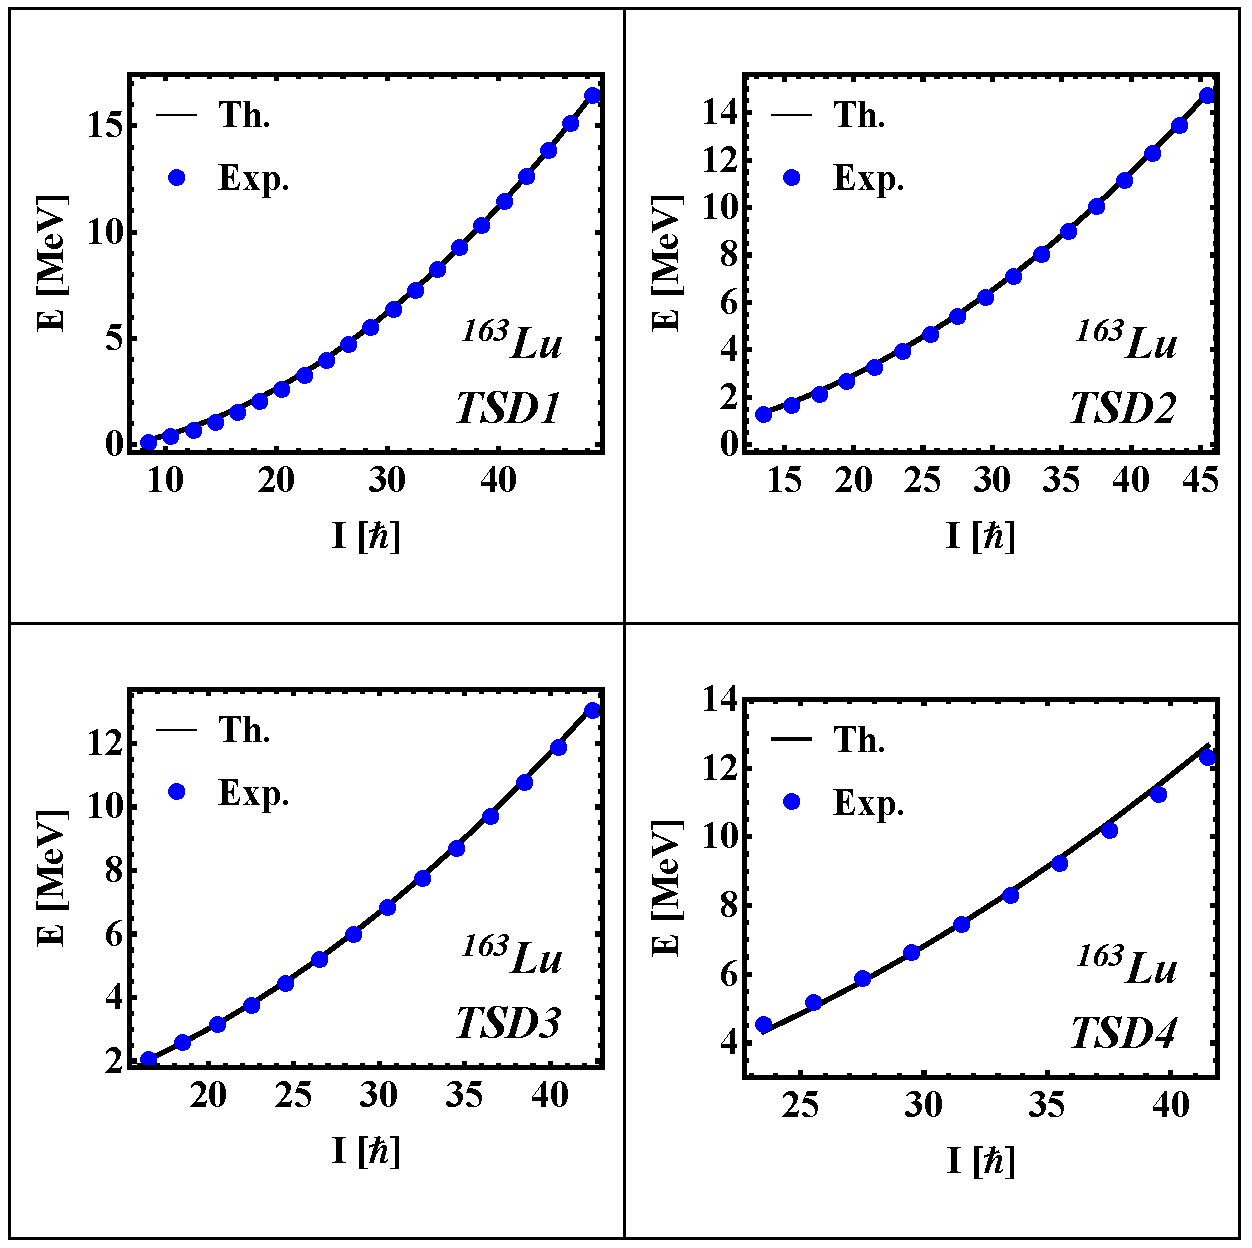
\includegraphics[scale=0.35]{ExcitationEnergies_GridView.pdf}
    \caption{The excitation energies for the wobbling spectrum of $^{163}$Lu. Comparison with the available experimental data.}
    \label{tsd_spectrum}
\end{figure}

The trajectories of a rotational state from $TSD_1$  is graphically represented in Figure \ref{trajectory}.

\begin{figure}[ht]
    \centering
    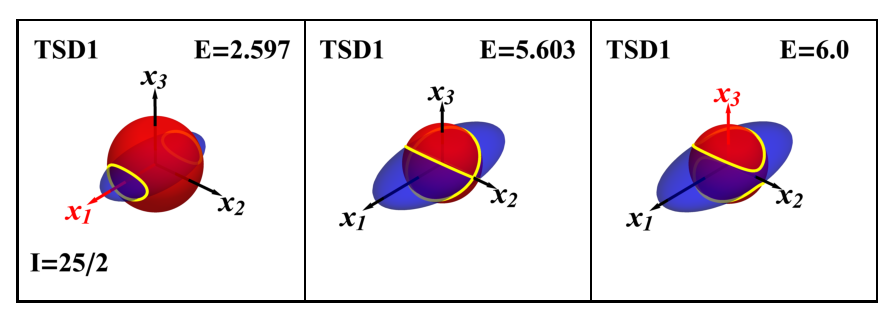
\includegraphics[scale=0.4]{tsd1_spin1.eps}
    \caption{The contour plots with the energy function $\mathcal{H}$ of the nucleus, evaluated for the obtained fit parameters.}
    \label{trajectory}
\end{figure}

The trajectories shown in Figure \ref{trajectory} are given by the intersection of two surfaces, namely the energy ellipsoid (generated from the expression of the energy function written in spherical coordinates) and the total angular momentum of the triaxial system. Each inset from the figure represents a trajectory at a given spin $I$ but different values of the total energy for the rotor. The first inset corresponds to the real energy of the isotope for that particular spin state. The second inset represents the energy at which the trajectories around 1-axis and -1-axis are tangent to each other. This particular energy marks the point of a phase transition, where the triaxial nucleus changes its rotational axis from 1-axis to the 3-axis. Finally, the third inset represents the trajectories belonging to very high energy states, where rotation is done around 3-axis. It is worth mentioning that such motion is forbidden for this isotope, since the energy at which the nucleus exhibits the 3-axis rotation is much larger than the excitation energy that corresponds to that particular spin.

A new interpretation on the wobbling motion, but based on the quasiparticle plus triaxial rotor model was given recently by Chen et. al. \cite{chen2020interpretation}.

\begin{acknowledgement}
We are grateful.
\end{acknowledgement}

\bibliography{references}

\end{document}